\documentclass[
  12pt,				    % tamanho da fonte
  openright,			% capítulos começam em pág ímpar (insere página vazia caso preciso)
  oneside,			  % para impressão em recto e verso. Oposto a oneside
  a4paper,			  % tamanho do papel. 
  hyphens,
  chapter=TITLE,  % títulos de capítulos convertidos em letras maiúsculas
  section=TITLE,  % títulos de seções convertidos em letras maiúsculas
  english,			  % idioma adicional para hifenização
  french,				  % idioma adicional para hifenização
  spanish,			  % idioma adicional para hifenização
  brazil				  % o último idioma é o principal do documento
]{iftex}

% Importa as macros do projeto
%% Macros de dados do documento
\autor{Nícolas Dezan dos Santos}
\titulo{AUTOMAÇÃO DE UM MALTEADOR LABORATORIAL: DESENVOLVIMENTO DE FIRMWARE E APLICATIVO PARA CONTROLE DE PROCESSOS}
\instituicao{Instituto Federal do Espírito Santo}
\newcommand{\campus}{Campus Vila Velha}
\newcommand{\imprimircampus}{\campus}
\curso{Curso de Química Industrial}
\local{Vila Velha-ES}
\data{2025}


\tipotrabalho{Trabalho de Graduação}
\preambulo{Trabalho de Conclusão de Curso apresentado à Coordenadoria do Curso de Química Industrial do
Instituto Federal de Educação, Ciência e Tecnologia do Espírito Santo, como requisito parcial para a obtenção do título de Químico Industrial.}

\orientador[Orientador][Prof. Dr.]{Ernesto}[Corrêa Ferreira]{Instituto Federal do Espírito Santo}
\coorientador[][]{}[]{}

\examinadori{Profa. Dra. Fulana de Tal}{Instituto Federal do Espírito Santo}{Examinadora} % DEPOIS
\examinadorii{Prof. Dr. Cicrano de Tal}{Instituto Federal do Espírito Santo}{Examinador} % DEPOIS

\approvaldate{32}{Dezembro}{2999} % DEPOIS

% Palavras-chaves
\palavraschave{Automação}[Malteação][Firmware][Engenharia de Alimentos][Controle de Processos]
\keywords{keyword 1}[keyword 2][keyword 3][keyword 4][keyword 5]

% Ficha catalográfica
\fichabiblioteca{
    Dados Internacionais de Catalogação-na-Publicação (CIP) \\
    (Biblioteca Nilo Peçanha do Instituto Federal do Espírito Santo) % Vish
}
\fichaautor{Elaborada por XXXXXXXXXXXXXXXXXXXXX – CRB-X/ES - XXX}
\fichatags{
    1. Redes neurais (Computação).  2. Expressão facial – Processamento de dados. 3. Sistemas de reconhecimento de padrões. 4. Processamento de imagens – Técnicas digitais. 5. Percepção de padrões. 6. Engenharia Elétrica. I. XXXXXXXX, XXXXXXXXXX XXXXXXXXXX.  II. Instituto Federal do Espírito Santo. III. Título.
}

\cutter{X999y}
\cdd{000.00}
\selectlanguage{brazil}

% Arial (para usar times-new-roman, comente as três linhas abaixo)
\usepackage{helvet}
\renewcommand{\familydefault}{\sfdefault}
\renewcommand{\ABNTEXchapterfont}{\bfseries}
% Comandos para revisar o texto
\usepackage{easyReview} 


%% Elementos opcionais
\editardedicatoria{\input{pre_textuais/dedicatoria}}
\editaragradecimentos{\input{pre_textuais/agradecimentos}}
\editarepigrafe{\input{pre_textuais/epigrafe}}


%% Listas [Siglas e Simbolos]
\editarlistasiglas{\input{pre_textuais/siglas}}
\editarlistasimbolos{\input{pre_textuais/simbolos}}

% Novos comandos
\newcommand{\ie}{\textit{i.e. }}
\newcommand{\eg}{\textit{e.g. }}



\begin{document}



  % --------------------------------------------------- %
  % CAPAS                                               %
  % --------------------------------------------------- %
  % CAPA E FOLHA DE ROSTO
  \capas
  \imprimircapa
  \imprimirfolhaderosto
  % \imprimirfichacatalografica
  % \includepdf[pages=-]{pre_textuais/ficha.pdf}

  % --------------------------------------------------- %
  % ELEMENTOS PRÉ-TEXTUAIS                              %
  % --------------------------------------------------- %
  % APROVAÇÃO, DEDICATÓRIA, AGRADECIMENTOS, EPÍGRAFE
  \pretextual
  % \imprimiraprovacao
  % \includepdf[pages=-]{pre_textuais/aprovacao.pdf}
  % \imprimirdedicatoria
  % \imprimiragradecimentos
  % \imprimirepigrafe
  
  % RESUMO - PT/EN
  % RESUMO - PT
\begin{resumo}
  \vspace{-15pt}
  
  A malteação é uma etapa crítica na produção de cerveja, exigindo o controle rigoroso de variáveis como temperatura, umidade e tempo ao longo das fases de maceração, germinação e secagem. Em ambientes acadêmicos, a ausência de equipamentos acessíveis e confiáveis limita o desenvolvimento de pesquisas nesta área. Este trabalho apresenta o desenvolvimento de um sistema de automação baseado no microcontrolador ESP32, com firmware programado em MicroPython e um aplicativo Android desenvolvido em Kotlin, capaz de monitorar e controlar o processo de malteação em laboratório. O sistema permite a configuração remota dos parâmetros de processo e o monitoramento em tempo real por meio da comunicação via Bluetooth Low Energy (BLE). A arquitetura do firmware foi estruturada com tarefas assíncronas independentes para controle de sensores, atuadores e etapas do processo. O aplicativo Android adota a arquitetura moderna em camadas (data, domain, presentation) com interface responsiva em Jetpack Compose, proporcionando usabilidade e modularidade. Os códigos desenvolvidos estão disponibilizados em repositórios GitHub, com o objetivo de promover reprodutibilidade e facilitar a adoção por outros pesquisadores. A solução proposta visa atender às demandas do LACEMP-IFES por uma plataforma de baixo custo e alta eficiência, contribuindo para a pesquisa aplicada em tecnologia de alimentos e automação de processos.

  Palavras-chave: \palavraschaveemlinha
\end{resumo}


% RESUMO - EN
\begin{resumo}[Abstract]
  \vspace{-15pt}
  
  \begin{otherlanguage*}{english}
    Malting is a critical stage in beer production, requiring strict control of variables such as temperature, humidity, and time during the steeping, germination, and kilning phases. In academic environments, the lack of accessible and reliable equipment limits research progress in this field. This work presents the development of an automation system based on the ESP32 microcontroller, with firmware programmed in MicroPython and an Android application developed in Kotlin, capable of monitoring and controlling the malting process in a laboratory setting. The system enables remote configuration of process parameters and real-time monitoring via Bluetooth Low Energy (BLE) communication. The firmware architecture was structured with independent asynchronous tasks to handle sensors, actuators, and process stages. The Android application adopts a modern layered architecture (data, domain, presentation) with a responsive interface built using Jetpack Compose, providing usability and modularity. The developed code is publicly available on GitHub, aiming to promote reproducibility and facilitate adoption by other researchers. The proposed solution addresses the demands of LACEMP-IFES for a low-cost and efficient platform, contributing to applied research in food technology and process automation.
  
  Keywords: \inlinekeywords
\end{otherlanguage*}
\end{resumo}
  
  % LISTAS E SUMÁRIO
  % \imprimirlistafiguras
  % \imprimirlistatabelas
  % \imprimirlistaquadros
  % \imprimirlistasiglas
  % \imprimirlistasimbolos
  \imprimirsumario

  % --------------------------------------------------- %
  % ELEMENTOS TEXTUAIS                                  %
  % --------------------------------------------------- %
  \textual
  \graphicspath{{figuras/}}   
  \chapter[Introdução]{Introdução}

O malte é um produto de extrema importância para diversos setores industriais, com ele sendo o principal insumo na produção de cerveja, onde fornece açúcares fermentáveis, cor e aroma à bebida. No setor cervejeiro, o malte de cevada é o mais utilizado; no entanto, há um crescente interesse em pesquisas que buscam desenvolver malte a partir de outros grãos, como arroz, milho e trigo, visando atender demandas específicas, como a produção de cervejas livres de glúten \cite{CECCARONI2019}. Além disso, o malte tem ganhado destaque como ingrediente funcional na indústria alimentícia, sendo utilizado, por exemplo, na fabricação de pães, devido às suas propriedades nutricionais \cite{KOISTINEN2020}.

A produção de malte, no entanto, enfrenta desafios significativos, especialmente em climas quentes, onde o controle preciso de temperatura, umidade e tempo, durante as etapas de maceração, germinação e secagem, é crucial para garantir a qualidade do produto \cite{KOVALOVA2024}. O controle desses parâmetros torna a malteação um processo complexo, exigindo equipamentos especializados e sistemas automatizados para otimizar a produção. No contexto acadêmico e de pesquisa, a falta de equipamentos acessíveis e confiáveis para malteação em laboratório limita o desenvolvimento de estudos e inovações nesta área, evidenciando a importância de soluções de baixo custo.
% A base dessa minha afirmação "forte" foram minhas pesquisas mais diretas por equipamentos, que normalmente são industriais. Essa é a forma que encontrei para justificar o trabalho, não sei se foi a melhor abordagem, mas parece funcionar. - Nicolas

Nesse contexto, um dos principais desafios enfrentados é a falta de equipamentos que permitam a malteação controlada em laboratório, comprometendo a precisão e a reprodutibilidade dos experimentos. Durante uma iniciação científica (IC), foi desenvolvido um protótipo inicial (\autoref{fig:malteador}), não finalizado, restando completar a montagem física e desenvolver o sistema de controle e automação. O presente trabalho dá continuidade à IC ao propor uma solução de \textit{software} responsável por garantir que o processo de malteação ocorra adequadamente. 
% A minha intenção é que essa última frase exponha os objetivos do trabalho. - Nicolas

\begin{figure}[ht]
    \centering
    \caption{Protótipo desenvolvido durante a IC. (A) Interface, placa de desenvolvimento e relés das válvulas; (B) Relé de estado sólido; (C) Parafuso de revolvimento; (D) Entrada de ar; (E) Entrada de água; (F) Saída de água; (G) Sensor de dióxido de carbono, umidade e temperatura.}  
    \label{fig:malteador}
    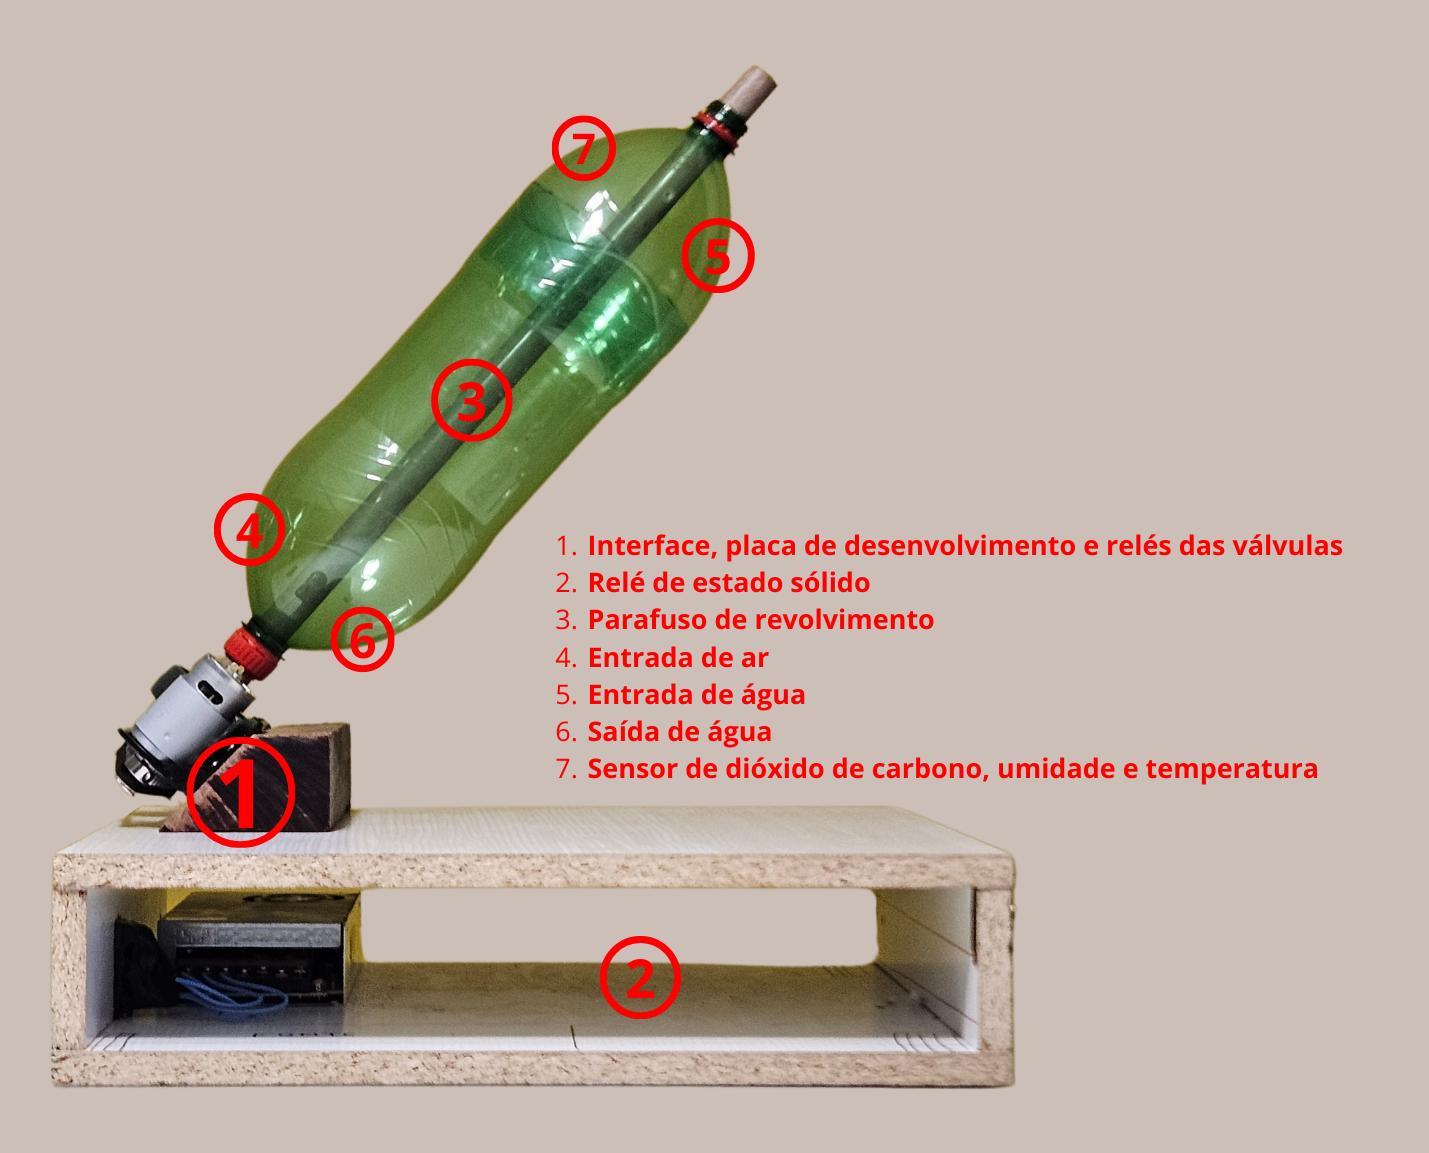
\includegraphics[width=0.8\textwidth]{Vista Lateral do Malteador.png}

    {\centering\footnotesize Fonte: Autoria própria.\par}
\end{figure}

A proposta visa o desenvolvimento de um sistema (\autoref{fig:esquemaeletronico}) baseado no microcontrolador ESP32-C3, da fabricante chinesa Espressif Systems, integrado com um aplicativo Android. Esse microcontrolador foi escolhido por sua relação custo-benefício, capacidade de processamento e suporte a tecnologias de comunicação como Bluetooth e Wi-Fi \cite{rodrigues2021controle, santos2019sistema}. Para seu firmware, optou-se pela linguagem MicroPython, que oferece uma curva de aprendizado suave e é bastante utilizada em projetos de prototipagem rápida e Internet das Coisas (IoT) \cite{TOLLERVEY2017, brito2020automaccao}. Já o aplicativo Android foi desenvolvido em Kotlin, linguagem oficial para o desenvolvimento Android \cite{sempreupdate_kotlin_2020}. A comunicação entre o firmware e o aplicativo é realizada via Bluetooth Low Energy (BLE), uma tecnologia de baixo consumo energético e amplamente disponível em dispositivos móveis \cite{heydon2012bluetooth}, permitindo a configuração remota e o monitoramento em tempo real dos parâmetros operacionais. Além disso, a documentação dos softwares desenvolvidos pode servir como referência para outros estudos envolvendo IoT dentro do IFES, especialmente no que se refere à integração entre ESP32 e Android.
% Adicionei referências a esse parágrafo. - Nicolas

\begin{figure}[ht]
    \centering
    \caption{Esquema eletrônico do malteador desenvolvido durante a IC: (A) relés para atuação das válvulas; (B) relés para atuação do motor e da resistência elétrica; (C) sensor de umidade, temperatura e dióxido de carbono; (D) painel LCD; (E) botão de emergência; (F) microcontrolador ESP32}
    \label{fig:esquemaeletronico}
    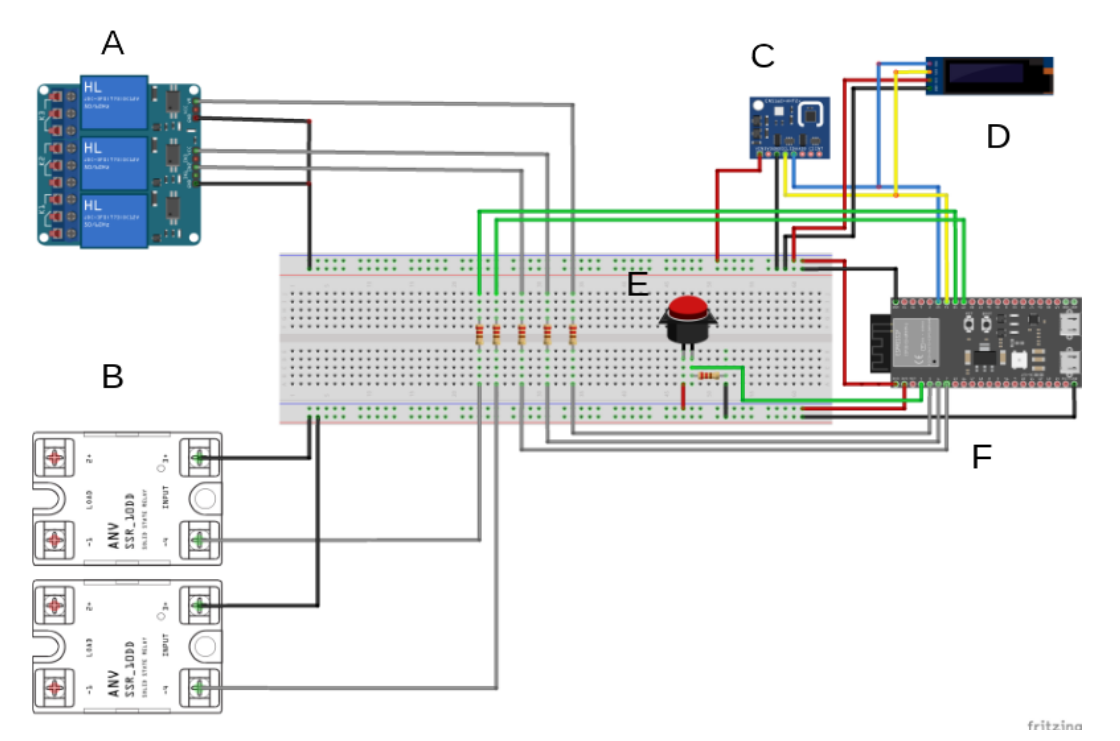
\includegraphics[width=0.8\textwidth]{esquemaeletronico.png}

    {\centering\footnotesize Fonte: Autoria própria.\par}
\end{figure}


Este trabalho surge a partir da demanda do Laboratório de Análises de Cerveja e Matérias-Primas (LACEMP), que busca iniciar estudos experimentais sobre o processo de malteação. A ausência de um equipamento adequado e acessível para pesquisas acadêmicas motivou o desenvolvimento de um sistema que permita monitorar e controlar as variáveis do processo de forma precisa e reprodutível. 

Por fim, a automação proposta busca simplificar a operação do equipamento e fornecer dados estruturados sobre o processo, facilitando futuras análises e ajustes nos experimentos conduzidos no LACEMP. Com isso, espera-se que esta solução de baixo custo promova avanços tanto na pesquisa acadêmica quanto no desenvolvimento de tecnologias acessíveis para a indústria cervejeira e áreas afins.
  \chapter[Referencial Teórico]{Referencial Teórico}

\section{O Processo de Malteação}

A malteação é um dos processos fundamentais na indústria cervejeira, responsável pela conversão do grão cru em um ingrediente essencial para a produção de cerveja. Esse processo ocorre em três etapas principais: maceração, germinação e secagem. Essas etapas são fundamentais para a produção de malte base: um malte que possui uma boa quantidade de enzimas e estoques de amido \cite{BRIGGS2004,CENCI2021}. Além disso, pode-se considerar uma quarta etapa no processo: a torrefação, que ocorre após a secagem e produz um malte especial no lugar de um malte base. Maltes especiais são conhecidos por serem formados com bastante influência das reações de Maillard \cite{COGHE2004}. A complexidade desse processo se dá no fato da manipulação de um organismo vivo, o grão, que exige controle rigoroso de suas condições de crescimento para se tornar um produto viável para comercialização \cite{MALLETT2022}. Além disso, em condições inadequadas de malteação, podem ocorrer ataques microbiológicos de diversas espécies, incluindo \textit{Fusarium sp.}, \textit{Penicillium} e \textit{Aspergillus genera} \cite{LUARASI2016}.

\subsection{Maceração}

Durante a maceração, com a submersão do grão em água, ocorre a liberação de hormônios e enzimas que darão início ao crescimento e desenvolvimento do grão \cite{LEWIS2012}. O teor de água no grão cresce rapidamente após o início dessa primeira etapa, que ocorre em duas fases distintas: uma inicial, em que o embrião e o escutelo absorvem água rapidamente, e uma segunda fase, mais lenta, em que o endosperma é gradualmente hidratado. Esse processo é crucial para a ativação de enzimas como a amilase, a ribonuclease e a fosfatase, que desempenham papeis essenciais na modificação do grão \cite{REYNOLDS1966}. Também é crucial que o oxigênio seja fornecido ao mesmo tempo em que o dióxido de carbono é eliminado dos grãos. O aumento da umidade intensifica o metabolismo do grão, elevando sua taxa respiratória, ou seja, mais oxigênio é requerido \cite{KUNZE1996}. Por isso, a presença de tanques de maceração que bombeiam ar através dos grãos submersos é frequente nas produções de larga escala \cite{CENCI2021}. Mas, muitos estudos ainda investigam os impactos de se trabalhar com ciclos de períodos secos e submersos, especialmente, quando se busca viabilizar novas variedades de grãos para a malteação \cite{MAYER2014,TURNER2019}.

\subsection{Germinação}

Ao fim da maceração, que pode durar até 72 horas, o teor de umidade dos grãos chega a aproximadamente 45\%, e as radículas tornam-se visíveis, indicando o momento adequado para o início da germinação. Essa segunda etapa é caracterizada por um elevado nível metabólico nos grãos, com a ocorrência de transformações bioquímicas essenciais para o processo de malteação \cite{MALLETT2022}. Do ponto de vista do malteador, a duração da germinação deve ser cuidadosamente controlada, pois um período insuficiente ou excessivo pode comprometer a qualidade do malte. Se a germinação for muito curta, as transformações necessárias nos grãos não ocorrerão de forma adequada. Por exemplo, as enzimas não conseguirão degradar completamente as paredes celulares proteicas que envolvem o amido, tornando-o menos disponível para as etapas subsequentes do processo cervejeiro \cite{FOX2009}. Por outro lado, uma germinação prolongada pode levar ao esgotamento excessivo dos nutrientes do grão visando o crescimento da planta, afetando negativamente o produto final \cite{LEWIS2012}.

Durante a germinação, a ativação de enzimas hidrolíticas desempenha um papel essencial na modificação do grão.As $\beta$-glucanases promovem a degradação dos $\beta$-glucanos presentes na parede celular do endosperma, substâncias estas que são indesejadas no processo cervejeiro em altas concentrações \cite{LEWIS2012}. Paralelamente, proteases hidrolisam a matriz proteica que envolve os grânulos de amido, liberando pequenos peptídeos e aminoácidos \cite{FOX2009,GUPTA2010}. Já a conversão do amido é mediada por enzimas amilolíticas,sendo a $\alpha$-amilase responsável pela quebra aleatória das ligações $\alpha$-1,4-glicosídicas e a $\beta$-amilase pela liberação de maltose, um dos principais açúcares fermentáveis do processo cervejeiro \cite{GUPTA2010,MALLETT2022}. Em essência, o grão cru entra no processo com compostos de alto peso molecular e, ao fim da malteação, gera como produto um malte com compostos de baixo peso molecular e boa concentração de enzimas \cite{KUNZE1996}. Essa transformação, que ocorre principalmente na germinação, é o que torna o malte indispensável para o processo cervejeiro \cite{CENCI2021}.

\subsection{Secagem}

Quando a germinação atinge o tempo otimizado para promover as melhores transformações, inicia-se a etapa de secagem. Nessa fase, de acordo com \apudonline{GRIFFITHS1992}{WOFFENDEN2002}, os grãos são desidratados por até 30 horas, o que resulta em um malte base de fácil manuseio e adequado para armazenamento. Além da redução da umidade para aumento da estabilidade do produto final, a secagem promove o desenvolvimento de aromas desejados e de coloração no malte \cite{BAMFORTH2003}. Apesar disso, se a intenção é produzir um malte base, a temperatura não pode ser excessiva, com o fim de preservar as enzimas, como as amilases, no produto final \cite{LEWIS2012}.Outra questão benéfica é que a secagem elimina boa parte dos microorganismos que cresceram de forma indesejada durante os processos anteriores \cite{DOUGLAS1988, PETTERS1988}. 


\section{Importância do controle de variáveis na malteação}

\subsection{Controle de temperatura}

O controle da temperatura durante a germinação é essencial para minimizar perdas causadas pelo crescimento excessivo das radículas e do embrião da planta, evitando o consumo desnecessário dos estoques de amido do grão \cite{PITZ1990, MALLETT2022}. Além disso, a temperatura influencia diretamente a atividade enzimática e a degradação de componentes estruturais do grão. Um estudo conduzido por \citeonline{BAXTER1980} avaliou os efeitos da maceração em uma temperatura superior à faixa usual de 12-16 $^{\circ}$C, chegando a 30 $^{\circ}$C. Os resultados indicaram que temperaturas elevadas comprometem a atividade enzimática e reduzem a eficiência da degradação de $\beta$-glucanos e proteínas, afetando negativamente a qualidade do malte.

Outro fator crítico relacionado à temperatura é o crescimento microbiológico. Segundo \citeonline{TANGNI2002}, temperaturas mais altas na malteação favorecem a proliferação de \textit{Aspergillus clavatus}, um fungo produtor de micotoxinas. A contaminação microbiológica ocorre predominantemente durante a germinação, mas também pode ser observada ao final da maceração \cite{PETTERS1988}. Dessa forma, a manutenção de temperaturas controladas entre 12 e 22 $^{\circ}$C durante as etapas de maceração e germinação é fundamental não apenas para garantir a qualidade do malte, mas também para assegurar a segurança sanitária do processo \cite{TANGNI2002}.

\subsubsection{Controle de temperatura na secagem}

Na etapa de secagem, o controle da temperatura desempenha um papel crucial em dois aspectos principais: garantir que o malte atinja a umidade adequada para armazenamento e determinar o tipo de malte produzido \cite{KUNZE1996}. A secagem ocorre, geralmente, em múltiplas fases, seguindo uma rampa de temperatura. Os valores típicos variam na faixa de 50 a 110 $^{\circ}$C, dependendo do perfil desejado para o malte final \cite{LEWIS2012}.

De acordo com \citeonline{SKENDI2018}, a temperatura de secagem influencia diretamente a composição de açúcares fermentáveis no malte e a coloração do mosto produzido. No estudo, a secagem a 80 $^{\circ}$C resultou em um mosto com maior teor de açúcares fermentáveis do que a secagem a temperaturas superiores, como 90 $^{\circ}$C. Além disso, foi observado um escurecimento do mosto com o aumento da temperatura de secagem, um fator determinante na definição das características finais do malte. Essa relação entre temperatura e cor ocorre devido à intensificação das reações de Maillard e à degradação térmica de compostos presentes no malte \cite{KUNZE1996}.

\subsection{Temp}
% Como temperatura, umidade e CO₂ afetam a qualidade do malte
  \chapter[Conclusão]{Conclusão}

Este trabalho apresentou o desenvolvimento de um sistema de automação para controle do processo de malteação em escala laboratorial, com base em uma arquitetura composta por \textit{firmware} para o microcontrolador \textit{ESP32-C3} e um aplicativo \textit{Android}. A proposta surgiu da necessidade identificada no \textit{LACEMP-IFES} por uma solução de baixo custo e com potencial didático, voltada ao estudo controlado da malteação em climas quentes.

O \textit{firmware} foi estruturado com lógica assíncrona, permitindo a execução simultânea de múltiplas tarefas, como leitura de sensores, controle de etapas e comunicação via \textit{Bluetooth Low Energy}. Por sua vez, o aplicativo \textit{Android}, desenvolvido em \textit{Kotlin}, adotou uma arquitetura modular em camadas, com funcionalidades que incluem envio de parâmetros, monitoramento em tempo real e gerenciamento de receitas.

Dentro do escopo estabelecido, os objetivos propostos foram alcançados: a comunicação \textit{BLE} entre os dispositivos foi implementada com sucesso, os algoritmos de controle das etapas de maceração, germinação e secagem foram desenvolvidos e validados por meio de simulações, e todo o código foi documentado e disponibilizado em repositórios públicos.

Embora validada por simulações, a solução não foi testada com o protótipo físico em funcionamento, uma vez que sua montagem completa e integração eletromecânica estavam fora do escopo deste trabalho. Assim, os testes com sensores e atuadores reais permanecem como uma etapa futura necessária para avaliar a performance prática da malteação realizada no equipamento.

Dessa forma, o trabalho cumpriu seu papel, entregando uma base funcional e bem documentada para o controle digital do processo. Apesar da ausência de testes com \textit{hardware} real, os resultados obtidos por simulação demonstram a viabilidade da proposta e oferecem um ponto de partida concreto para desenvolvimentos futuros.
  \chapter{Testes}  
\label{chap: testes}

\section{Dummy text com figuras}

Lorem ipsum dolor sit amet, consectetuer adipiscing elit. Aenean commodo ligula eget dolor. Aenean massa. Cum sociis natoque penatibus et magnis dis parturient montes, nascetur ridiculus mus. Donec quam felis, ultricies nec, pellentesque eu, pretium quis, sem. Nulla consequat massa quis enim. Donec pede justo, fringilla vel, aliquet nec, vulputate eget, arcu. In enim justo, rhoncus ut, imperdiet a, venenatis vitae, justo. Nullam dictum felis eu pede mollis pretium.

Lorem ipsum dolor sit amet, consectetuer adipiscing elit. Aenean commodo ligula eget dolor. Aenean massa. Cum sociis natoque penatibus et magnis dis parturient montes, nascetur ridiculus mus. Donec quam felis, ultricies nec, pellentesque eu, pretium quis, sem. Nulla consequat massa quis enim. Donec pede justo, fringilla vel, aliquet nec, vulputate eget, arcu. In enim justo, rhoncus ut, imperdiet a, venenatis vitae, justo. Nullam dictum felis eu pede mollis pretium.

\begin{figure}[ht]
  \caption{Mãe, eu formei!}
  \label{fig: fig1}
  \centering
  \includegraphics[width=0.7\textwidth]{graduation.png}
  \legend{Google images}
  
\end{figure}

\begin{figure}[ht]
  \caption{Ferramentas utilizadas}
  \label{fig: fig2}
  \centering
  \subfloat[overleaf\label{subfig: fig2a}]{\includegraphics[width=0.3\textwidth]{overleaf.png}}
  \hfill
  \subfloat[latex\label{subfig: fig2b}]{\includegraphics[width=0.3\textwidth]{latex.png}}
  \hfill
  \subfloat[github\label{subfig: fig2c}]{\includegraphics[width=0.3\textwidth]{github.png}}
  \legend{Google images}
  
\end{figure}

Integer tincidunt. Cras dapibus. Vivamus elementum semper nisi. Aenean vulputate eleifend tellus. Aenean leo ligula, porttitor eu, consequat vitae, eleifend ac, enim. Aliquam lorem ante, dapibus in, viverra quis, feugiat a, tellus. Phasellus viverra nulla ut metus varius laoreet. Quisque rutrum. Aenean imperdiet. Etiam ultricies nisi vel augue. Curabitur ullamcorper ultricies nisi. Nam eget dui. Etiam rhoncus. Maecenas tempus, tellus eget condimentum rhoncus, sem quam semper libero, sit amet adipiscing sem neque sed ipsum. Nam quam nunc, blandit vel, luctus pulvinar, hendrerit id, lorem. Maecenas nec odio et ante tincidunt tempus. Donec vitae sapien ut libero venenatis faucibus. Nullam quis ante. Etiam sit amet orci eget eros faucibus tincidunt. Duis leo. Sed fringilla mauris sit amet nibh. Donec sodales sagittis magna. Sed consequat, leo eget bibendum sodales, augue velit cursus nunc,

\subsection{Tabelas e Quadros}

Segue exemplos de como usar tabelas e quadros.

\begin{table}[ht]
  \caption{Faixa etária dos alunos (número e proporção) do Curso de Saneamento do Ifes – Campus Vitória no no de 2016.}
  \label{tab: table1}
  \centering

  \begin{tabular}{ccc}
    \hline
    \bfseries Faixa Etária & \bfseries Número & \bfseries Porcentagem\\
    \hline
    18 a 25 & 7 & 25,7 \\
    26 a 30 & 25 & 70,3 \\
    31 a 40 & 2 & 3,0 \\
    40 a 50 & 1 & 1,0 \\
    + de 50 & - & - \\
    \hline
    Total & 35 & 100 \\
    \hline
  \end{tabular}

  \source
\end{table}
  
\begin{quadro}[ht]
  \caption{Configuração de microcomputador XP.}
  \label{quad: quadro1}
  \centering
  
  \begin{tabularx}{\textwidth}{lX}
    \hline
    \bfseries Elemento & \bfseries Especificações\\
    \hline
    1 CD & CD + Disk Driver para apenas uma entrada de disquete \\
    Kit de multimídia 8X & Kit com placa de som, caixas, microfone, CD-ROM com velocidade 8X e títulos \\
    8 Mb RAM & Quantidade de memória RAM (ver memória) \\
    66 Mhz & Velocidade do computador \\
    PC 486 DX/2 & Tipo e modelo do computador \\
    840 Mb HD & Capacidade de armazenamento do computador \\
    \hline
  \end{tabularx}

  \legend{Barbosa (1999 apud UFES, 2004)}
\end{quadro}

\subsubsection{Teste com referências}

Segue abaixo uma lista de referências:

\begin{itemize}%[nosep]
  \item Referência cruzada com capítulos: \autoref{chap: testes}
  \item Referência cruzada com anexos: \refanexo{anexo: a}
  \item Referência cruzada com apêndices: \refapendice{apendice: a}
  \item Referência cruzada com figuras: \autoref{fig: fig1}
  \item Referência cruzada com sub-figuras: Figura \ref{subfig: fig2a}
  \item Referência cruzada com tabelas: \autoref{tab: table1}
  \item Referência cruzada com quadros: \autoref{quad: quadro1}
  \item Referência cruzada com equações: \autoref{eq: eq1}
\end{itemize}
    
\subsubsubsection{Equações e Códigos}

O Teorema de Pitágoras é dado por:

\begin{equation}
    \label{eq: eq1}
	a^{2}= b^{2}+c^{2}
\end{equation}

Exemplo de código de programação:
  
\lstinputlisting[language=Python, caption=Perceptron]{algoritmos/perceptron.py} % Deletar arquivo textuais/testes.tex
      
  % --------------------------------------------------- %
  % ELEMENTOS POS-TEXTUAIS %
  % --------------------------------------------------- %
  \postextual
  
  % Referencias Bibliográficas
  \bibliographystyle{abntex2-alf} % Autor-Data
  \bibliography{bibliografia}
    
  % Apêndices
  \begin{apendicesenv}
    \input{pos_textuais/apendice.tex}
  \end{apendicesenv}

  % Anexos
  \begin{anexosenv}
    \input{pos_textuais/anexo.tex}
    \input{pos_textuais/easyreview.tex}
  \end{anexosenv}

  % Índice Remissivo
  \phantompart
  \printindex

\end{document}